\documentclass{article}
\usepackage[utf8]{inputenc}
\usepackage[T1]{fontenc}
\usepackage[polish]{babel}
\usepackage{graphicx}
\title{Pierwszy rozdział}
\author{Jakub Olech}
\date{15 November 2022}
\begin{document}
\maketitle
\begin{center}
Najpiękniejszy wzór w matematyce
\end{center}
\[ e^{i\pi} + 1 = 0 \]

\section{Zdjęcie:}

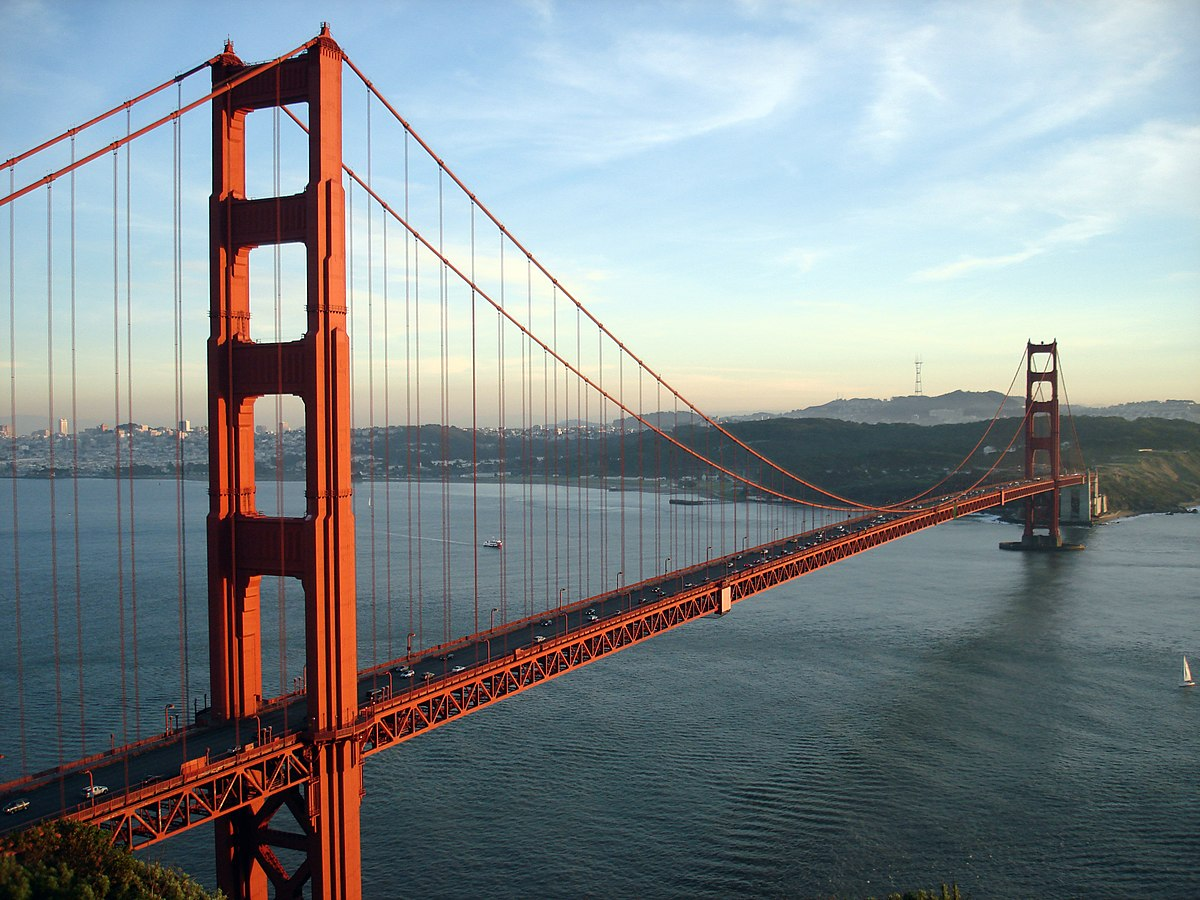
\includegraphics[width=5cm]{pictures/GoldenGateBridge.jpg}

\section{Tabela:}

\begin{tabular}{llllllll}
A & B & C & D & E & F & G & H \\
3 & 1 & 4 & 1 & 5 & 9 & 2 & 6 \\
5 & 3 & 5 & 9 & - & - & - & - \\
- & - & - & - & - & - & - & -
\end{tabular}

\section{Lista numerowana:}
\label{sec:lista}
\begin{enumerate}
    \item Item1
    \item Item2
    \item Item3
\end{enumerate}

\par

\section{Lista nienumerowana}
\label{sec:lista}
Jest to sekcja numer~\ref{sec:lista}
\begin{itemize}
    \item Item1
    \item[-] Item2
    \item[*] Item3
\end{itemize}

\section{Paragraf z podstawowym formatowaniem}
\begin{flushleft}
\textbf{Lorem ipsum dolor sit amet}, consectetur adipiscing elit, sed do eiusmod tempor incididunt ut labore et dolore magna aliqua.
\end{flushleft}
\begin{center}
Ut enim ad minim veniam, \underline{quis nostrud exercitation ullamco laboris nisi ut aliquip ex ea} commodo consequat.    
\end{center}
\begin{flushright}
Duis aute irure dolor in \emph{reprehenderit in voluptate} velit esse cillum dolore eu fugiat nulla pariatur.
\end{flushright}

\end{document}